%-*-EMaxima-*-

In addition to some options with respect to the mathematical output from Maxima
on the command line, the system is also capable of interfacing with external
programs to provide graphing capabilities.  You can also save Maxima sessions 
to reload later.


\section{Options on the Command Line}

While for normal use the default settings are likely to be preferable, Maxima 
allows you to set some options with regards to how output is returned.  

\subsection{1D vs. 2D}

The default output Maxima gives you when you evaluate an expression is 2D 
output, which basically means you have some visual feedback on the structure
of things like fractions and integrals as ascii art, and the output expression
is not one string.  Normally this is a good thing, but if for any reason you 
wish to turn that feature off, it is quite possible to do so.  Maxima has an
internal variable regulating this feature called \texttt{DISPLAY2D}.  
Ordinarily it is set to TRUE, providing the typical ascii Maxima output you
would get in a terminal session.  Setting it to FALSE will cause returns to
be a single string.  Here is an example:

\beginmaximasession
2*y*3*x/(4*x+y+3/4);
DISPLAY2D:FALSE;
2*y*3*x/(4*x+y+3/4);
\maximasession
(C1) 2*y*3*x/(4*x+y+3/4);

                                     6 x y
(D1)                              -----------
                                            3
                                  y + 4 x + -
                                            4
(C2) DISPLAY2D:FALSE;

(D2) FALSE
(C3) 2*y*3*x/(4*x+y+3/4);

(D3) 6*x*y/(y+4*x+3/4)
\endmaximasession

One important note here is that if you only wish to change the dimension
of your output for one entry, you must set this variable by hand both
before and after the command - i.e., \texttt{ev(2/3,DISPLAY2D:FALSE)} will
not result in \texttt{2/3} unless the DISPLAY2D:FALSE command has already
been entered - ev will not use it in its evaluation.

\subsection{TeX Strings as Output}

As you probably already know, Maxima is able to output expressions in TeX
format.  This ability is used transparently in several places, but you can
also request this output manually, using the \texttt{tex(expression)} command.

\beginmaximasession
A1:integrate(2*x+x^3+3*x^2,x);
tex('integrate(sin(x)/(2*x+x^3+3*x^2),x));
tex(A1);
\maximasession
(C5) A1:integrate(2*x+x^3+3*x^2,x);

                                  4
                                 x     3    2
(D5)                             -- + x  + x
                                 4
(C6) tex('integrate(sin(x)/(2*x+x^3+3*x^2),x));

$$\int {{{\sin x}\over{x^{3}+3\>x^{2}+2\>x}}}{\>dx}$$
(D6)                                 FALSE
(C7) tex(A1);

$${{x^{4}}\over{4}}+x^{3}+x^{2}$$
(D7)                                 FALSE
\endmaximasession

This is useful if you are writing a paper without the benefit of Emaxima
and wish to include a Maxima result - the above can be pasted directly
into a LaTeX environment.

\subsection{Writing a Session to a File}

This is actually a bit tricky, especially if you decide halfway through
a session you wish to make a record of it.  Fortunately, however, there
are some tools you can use. 

Note:  Need to figure out the subtlties of save()

\subsubsection{Writefile}

The basic command you will want to start running when you want to record
a session.  The syntax works like this: \verb@writefile("/home/user/maxima@
 \verb@sessionoutput.txt")$@

This will record the entire session into a text file called \texttt{maximasessionoutput.txt} in the \texttt{/home/user} directory.  If you wish close this
file, you simply use the command \verb@closefile("/home/user/maxima@ \verb@sessionoutput.txt")$@  These files are not loadable as commands - it is merely
a transcript of a session as it occurred.  This is useful for basic text
documentation preperation, or just basic saving of a session for printing.

If you wish to record lines that were entered before you began writing the file to 
disk, you can use a command called \texttt{PLAYBACK} to get them into the record.
(Discuss playback options here.)

\subsubsection{Creating BATCHable files - Stringout}

If the user wishes to create a file containing session information which may be loaded again into the system using the BATCH, then \texttt{STRINGOUT} is the command you want to use.  There are several choices here - you can save specific input (listing C labels), include all C input lines by supplying the arguement INPUT, all of the functions you have defined by supplying the argument FUNCTIONS, and also all the values you have defined by supplying the arguement VALUES.
Since this is potentially quite important in the creation of packages and specialized invironments, we will go into this with some detailed examples.

Let's imagine we want to create a package to calculate the volume of a cube, with certain default values in place.  We begin by entering these
commands in Maxima:

\beginmaximasession
defaultlength:35$
defaultheight:45$
defaultwidth:65$
volume(length,width,height):=length*width*height;
defaultvolume:volume(defaultlength,defaultwidth,defaultheight)$
defaultvolume;
\maximasession
(C1) defaultlength:35$

(C2) defaultheight:45$

(C3) defaultwidth:65$

(C4) volume(length,width,height):=length*width*height;

(D4)         volume(LENGTH, width, height) := LENGTH width height
(C5) defaultvolume:volume(defaultlength,defaultwidth,defaultheight)$

(C6) defaultvolume;

(D6)                                102375
\endmaximasession

Of course, the last line is not strictly necessary, but it will serve to illustrate the difference between various options.  Now, as a first example we will save all the lines of input to the file cube.mac:

\beginmaximasession
stringout("cube.mac",INPUT);
\maximasession
(C7) stringout("cube.mac",INPUT);

(D7)       /home/user/cube.mac
\endmaximasession

Notice the return from this command is the directory where the file is located.  If we look at the contents of that file:

~

\begin{verbatim}
defaultlength:35$
defaultheight:45$
defaultwidth:65$
volume(LENGTH,width,height):=LENGTH*width*height;
defaultvolume:volume(defaultlength,defaultwidth,defaultheight)$
defaultvolume;
\end{verbatim}

~

We see that this is the series of commands we entered.  If we were to load
this file with the \texttt{batch} command (reference this somewhere) we would get precisely the same thing we got before.  Now let's try the FUNCTIONS and VALUES arguements:

\beginmaximasession
stringout("cubefunctions.mac",FUNCTIONS);
stringout("cubevalues.mac",VALUES);
\maximasession
(C8) stringout("cubefunctions.mac",FUNCTIONS);

(D8)   /home/user/cubefunctions.mac
(C9) stringout("cubevalues.mac",VALUES);

(D9)    /home/user/cubevalues.mac
\endmaximasession

And we see the contents of those files are:

\begin{verbatim}

cubefunctions.mac

volume(LENGTH,width,height):=LENGTH*width*height;
\end{verbatim}


\begin{verbatim}

cubevalues.mac

defaultlength:35;
defaultheight:45;
defaultwidth:65;
defaultvolume:102375;
\end{verbatim}

~

So those are the basics of how output works.  Experiment a little before you
begin creating batch files, so you know in more detail what is saved and
what isn't by various options.  In the case of FUNCTIONS, the following
will tell you what you have defined:

\beginmaximasession
DISPFUN(ALL);
\maximasession
(C10) DISPFUN(ALL);

(E10)        volume(LENGTH, width, height) := LENGTH width height

(D10)                                DONE
\endmaximasession

You will also want to examine the \texttt{VALUES} variable and the use of 
the \texttt{PACKAGEFILE} variable.

\newpage

\section{Graphics}

Maxima has, via external programs, the ability to produce 2D and 3D graphs.  The information will also be recorded in a file called maxout.openmath.  The information in that file will always be the raw openmath format data of the last plot command.

\subsection{2D function plotting}

2D graphs are produced with the \texttt{plot2d} command.  Perhaps the simplest way to introduce this
command is to show it in action.

~\\
\verb@plot2d([sin(x),cos(x),tan(x)],[x,0,2*%Pi],[y,-1,1]);@\\
~\\
{\centering 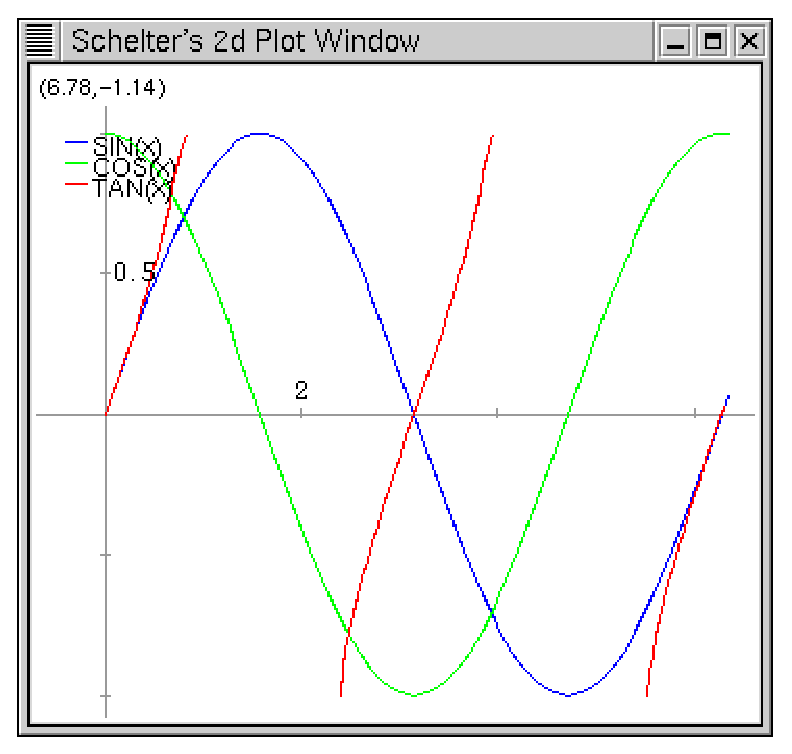
\includegraphics{images/2dplotwindow} \par }

~

These are just the basics - there are many options which can be set, but most of them are part of an overall plot options system which we will discuss later.  In the examples section at the end of this chapter we will show some more 2D plots with various options set.

\subsection{3D Function Plotting}

This works just about like the 2D plotting, only you need to supply the proper parameters.  Here again an example is the best teacher.

~\\
\verb@Plot3d(r^.33*cos(th/3),[r,0,1],[th,0,6*%pi],['grid,12,80],@\\
\verb@['transform_xy,polar_to_xy],['view_direction,1,1,1.4],['colour_z,true]);@\\
~\\
{\centering 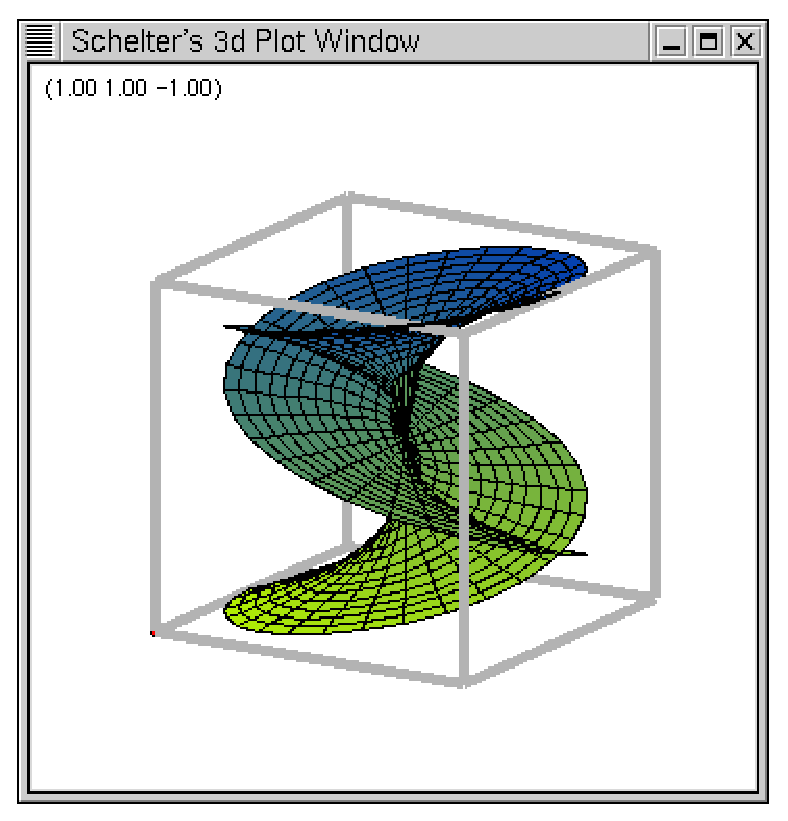
\includegraphics{images/3dplotwindow} \par }

~

Notice in the latter shot the control menu is visible - this appears if you move the mouse to the upper left hand corner of the plot window, and will allow you to configure things like printing options.

\section{Plot Options}



Maxima defines a list, called \verb@PLOT_OPTIONS@, which controls most of the behavior of Maxima's plotting options.  There are two ways of setting these options - you can set an option globally, using the \verb@SET_PLOT_OPTION@ command \footnote{Setting an option globally only changes the option for the current Maxima session - upon restart, the original defaults will be restored.}, or supply the new options as arguements to a plot command.  If you want to check what your global options are currently set at, you can just type \verb@PLOT_OPTIONS;@ and the current state of the system will be listed.

\beginmaximasession
PLOT_OPTIONS;
\maximasession
(C1) PLOT_OPTIONS;

(D1) [[x, - 3, 3], [y, - 3, 3], [GRID, 30, 30], [VIEW_DIRECTION, 1, 1, 1], 

[COLOUR_Z, FALSE], [TRANSFORM_XY, FALSE], [RUN_VIEWER, TRUE], 

[PLOT_FORMAT, OPENMATH], [NTICKS, 100]]
\endmaximasession

OK, let's look at each of these options.

\begin{itemize}
  \item \verb@[x, - 3, 3]@ - This defines the X range.  In order to change this range globally, use a command of the form \verb@SET_PLOT_OPTION([x,-5,5]);@
  \item \verb@[y, - 3, 3]@ - This defines the Y range.  In order to change this range globally, use a command of the form \verb@SET_PLOT_OPTION([y,-5,5]);@
  \item \verb@[GRID, 30, 30]@ - This controls, in 3D plotting, the number of points used to draw the figure.  The function is only calculated at a certain number of points - after that, linear approximations are drawn. Globally, usee a command of the form \verb@SET_PLOT_OPTION([GRID,40,35]);@
  \item \verb@[VIEW_DIRECTION, 1, 1, 1]@ - This option is specific to the case
  when the plot command outputs directly to postscript in 3D(See
  \verb@PLOT_FORMAT@.)  It determines the direction from which the 'camera'
  looks at the function, which is along a line parallel to the line from
  \verb@VIEW_DIRECTION@ to the origin.  It only needs to be set in the case of
  postscript output; it is ignored otherwise.  Globally, use a command of the
  form \verb@SET_PLOT_OPTION([VIEW_@ \verb@DIRECTION,1.4,1.4,1.4]);@
  \item \verb@[COLOUR_Z, FALSE]@ - This refers also to the postscript output - if set to TRUE it provides a little color shading in the output. Form is \verb@SET_PLOT_OPTION([COLOUR_Z, TRUE]);@
  \item \verb@[TRANSFORM_XY, FALSE]@ - This appears to provide the ability to produce plots with different coordinate systems, but I am unsure of how to make it work.  Need to get help here.
  \item \verb@[RUN_VIEWER, TRUE]@ - If you only wish Maxima to output the openmath file and not launch the graphical viewer, set this option to false.  Remember, however, that if you wish to run multiple commands to generate data you will have to recover the information from the maxout.openmath file each time, because each new plot command will overwrite it. Form is \verb@SET_PLOT_OPTION([RUN_VIEWER, FALSE]);@
  \item \verb@[NTICKS, 100]@ - Controls the number of points used to draw the 2D plots - the program will calculate the value of the function at N points, and then draw lines between them.  Form is \verb@SET_PLOT_OPTION([NTICKS, 200]);@
  \item \verb@[PLOT_FORMAT, OPENMATH]@ - This controls which program gets the output from Maxima for display.  There are currently four viable options - OPENMATH, GNUPLOT, GEOMVIEW, and PS.  PS is simply direct output to a postscript file, maxout.ps.  All of these programs are freely available.  
  Geomview is currently Unix only, and is available at
  http://geomview.sourceforge.net as both source and binary.  Openmath is
  distributed as part of Maxima.  Gnuplot is widely available, with a homepage
  at http://www.gnuplot.org and the most current development version at
  http://sourceforge.net/projects/gnuplot.  Gnuplot can run on both Windows and
  Linux. 
  \end{itemize}

\begin{figure}

\centering 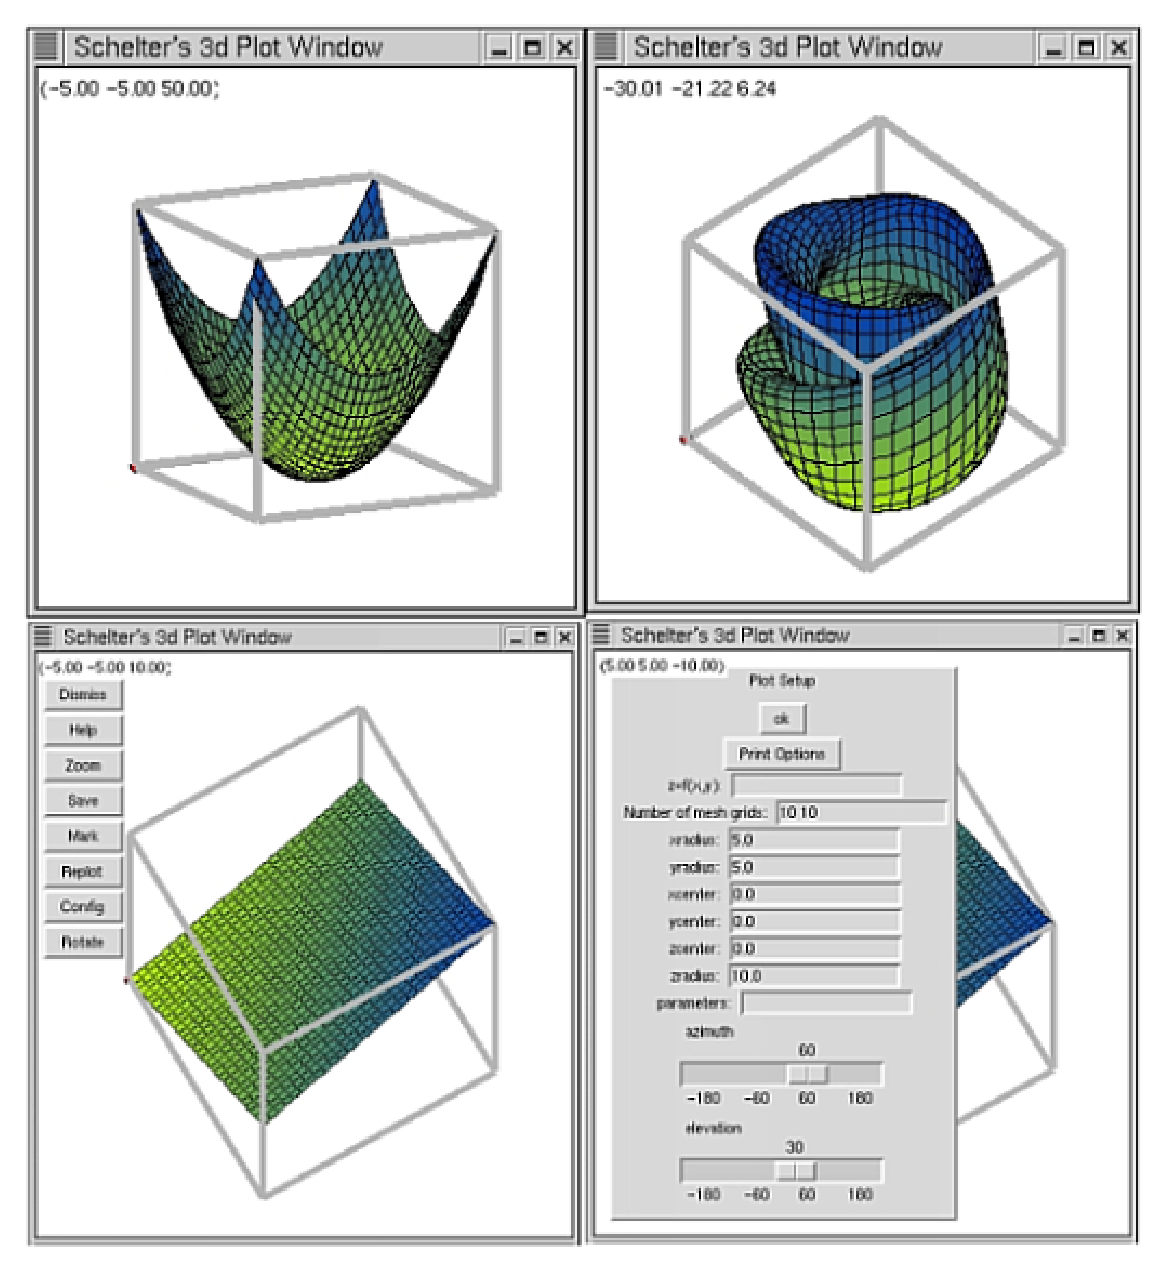
\includegraphics{images/maxima_openmath} \par
\caption{Graphing with Openmath, the default Maxima plotting tool}

\end{figure}

\begin{figure}

\centering 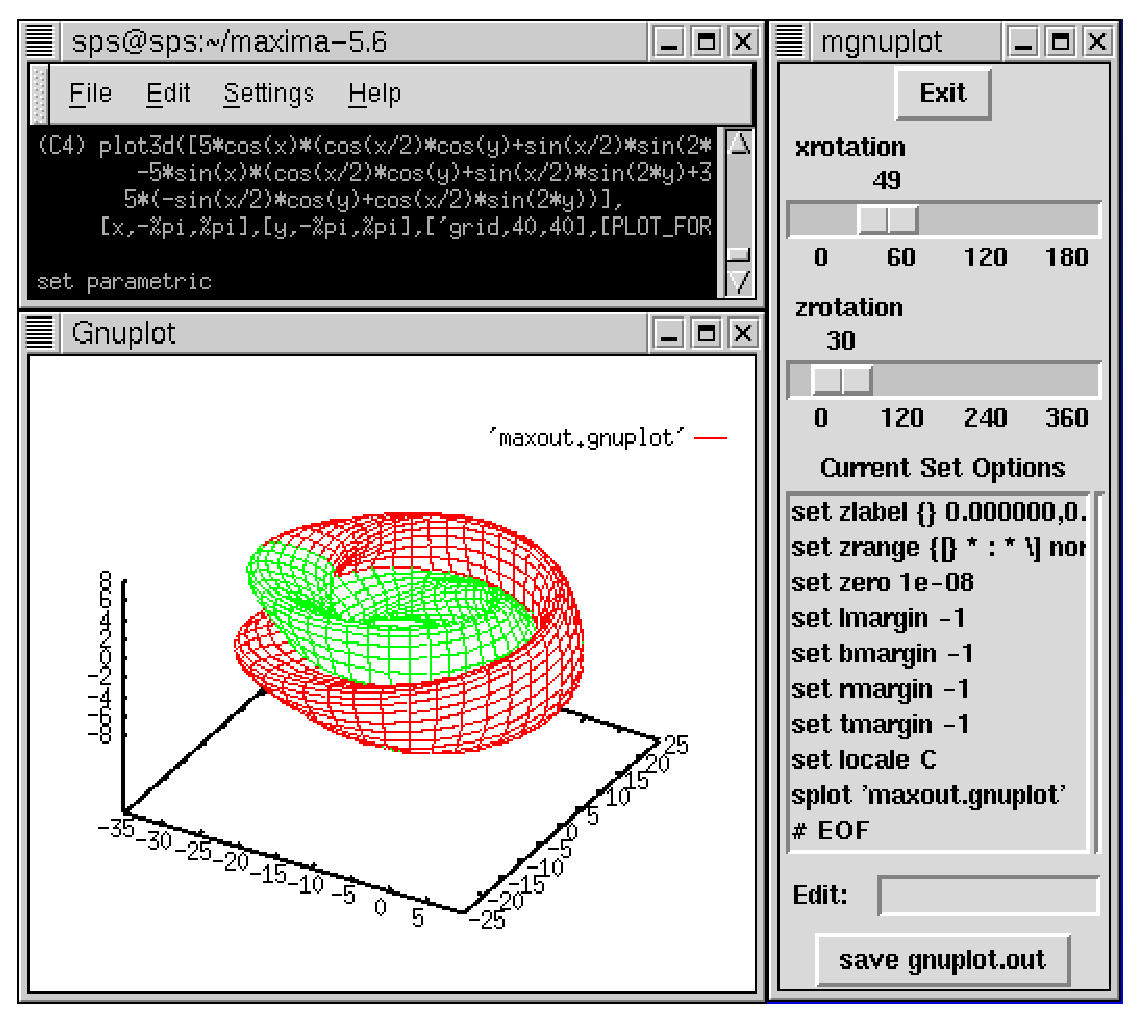
\includegraphics{images/maxima_gnuplot} \par
\caption{Graphing with gnuplot, using the mgnuplot utility}

\end{figure}


\begin{figure}

\centering 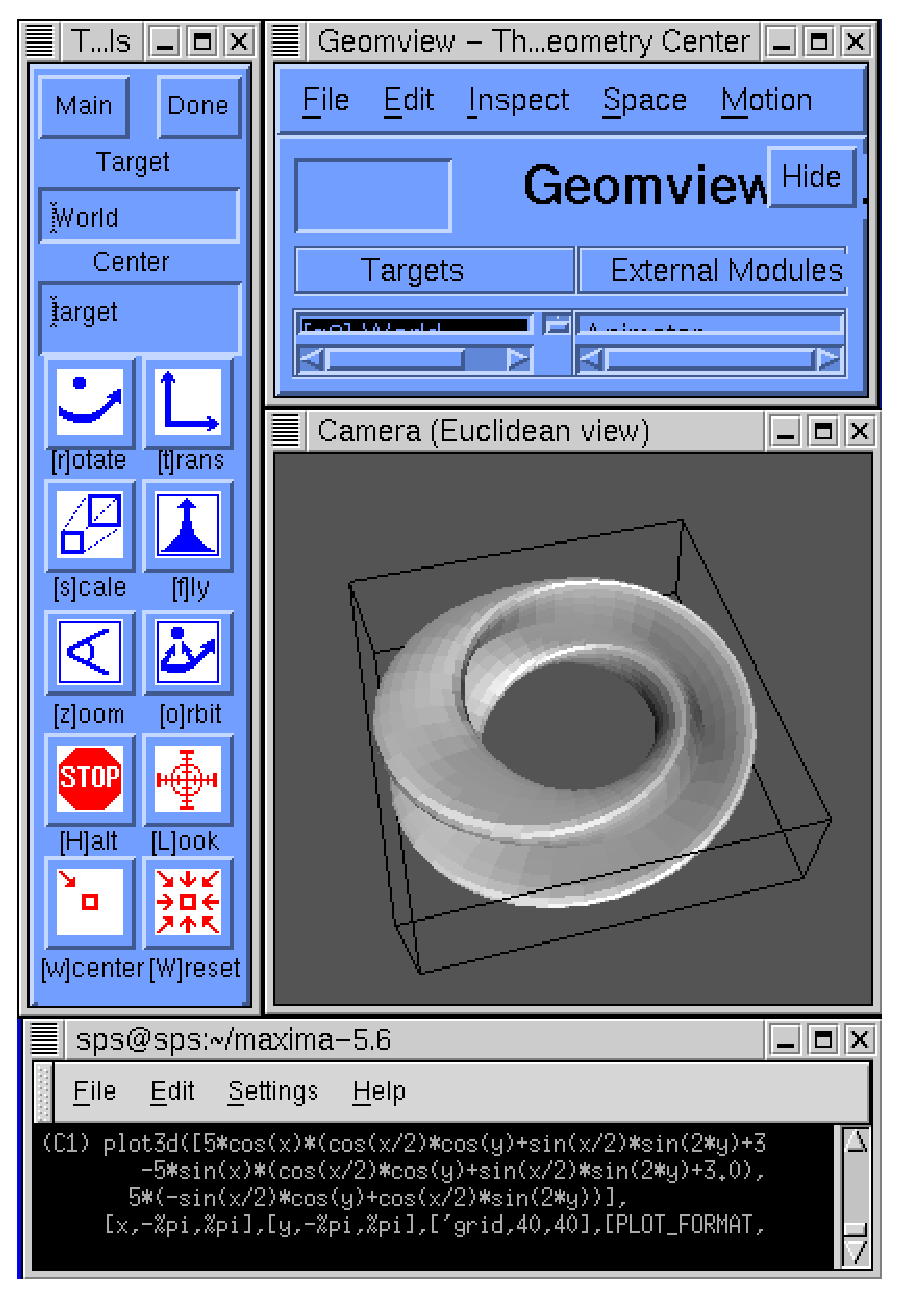
\includegraphics{images/maxima_geomview} \par
\caption{Graphing with GeomView.}

\end{figure}


